\documentclass[12pt,letterpaper]{article}
\usepackage[utf8]{inputenc}
\usepackage[spanish]{babel}
\usepackage{graphicx}
\usepackage[left=2cm,right=2cm,top=2cm,bottom=2cm]{geometry}
\usepackage{graphicx} % figuras
% \usepackage{subfigure} % subfiguras
\usepackage{float} % para usar [H]
\usepackage{amsmath}
%\usepackage{txfonts}
\usepackage{stackrel} 
\usepackage{multirow}
\usepackage{enumerate} % enumerados
\renewcommand{\labelitemi}{$-$}
\renewcommand{\labelitemii}{$\cdot$}
% \author{}
% \title{Caratula}
\begin{document}

% Fancy Header and Footer
% \usepackage{fancyhdr}
% \pagestyle{fancy}
% \cfoot{}
% \rfoot{\thepage}
%

% \usepackage[hidelinks]{hyperref} % CREA HYPERVINCULOS EN INDICE

% \author{}
\title{Caratula}

\begin{titlepage}
\begin{center}
\large{UNIVERSIDAD PRIVADA DE TACNA}\\
\vspace*{-0.025in}
\begin{figure}[htb]
\begin{center}

\includegraphics[width=8cm]{./Imagenes/logo}
\end{center}
\end{figure}
\vspace*{0.15in}
INGENIERIA DE SISTEMAS  \\

\vspace*{0.5in}
\begin{large}
TITULO:\\
\end{large}

\vspace*{0.1in}
\begin{Large}
\textbf{INFORME DE LABORATORIO No. 05} \\
\end{Large}

\vspace*{0.3in}
\begin{Large}
\textbf{CURSO:} \\
\end{Large}

\vspace*{0.1in}
\begin{large}
INTELIGENCIA DE NEGOCIOS\\
\end{large}

\vspace*{0.3in}
\begin{Large}
\textbf{DOCENTE:} \\
\end{Large}

\vspace*{0.1in}
\begin{large}
Ing. Patrick Cuadros Quiroga\\
\end{large}

\vspace*{0.2in}
\vspace*{0.1in}
\begin{large}
Integrantes: \\
\begin{flushleft}


Acosta Ortiz,Orlando Antonio  \hfill	(2015052775) \\

\end{flushleft}
\end{large}
\end{center}

\end{titlepage}


\tableofcontents % INDICE
\thispagestyle{empty} % INDICE SIN NUMERO
\newpage
\setcounter{page}{1} % REINICIAR CONTADOR DE PAGINAS DESPUES DEL INDICE

\section{Actividad 01: Importación de datos usando el Wizard - Sql Managment} 

1. Crearemos una base de datos llamada BDTEST\\
	\begin{center}
	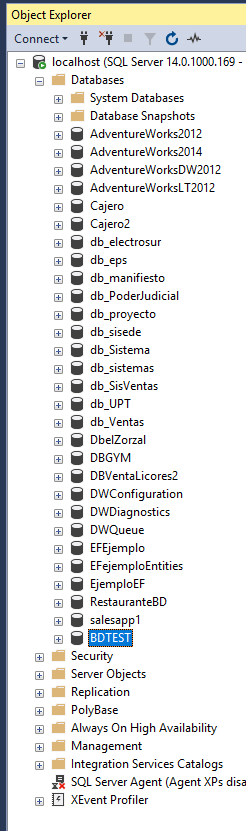
\includegraphics[width=7cm,height=21cm]{./Imagenes/img1}
	\end{center}	


2.  Importamos la  base de datos desde AdventureWorks.\\
	\begin{center}
	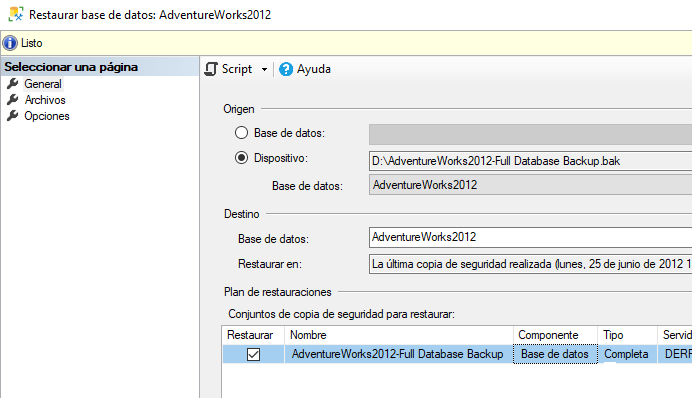
\includegraphics[width=11cm]{./Imagenes/img2}
	\end{center}	
\pagebreak
3. Escribir el Servidor y seleccionar la base de datos\\
	\begin{center}
	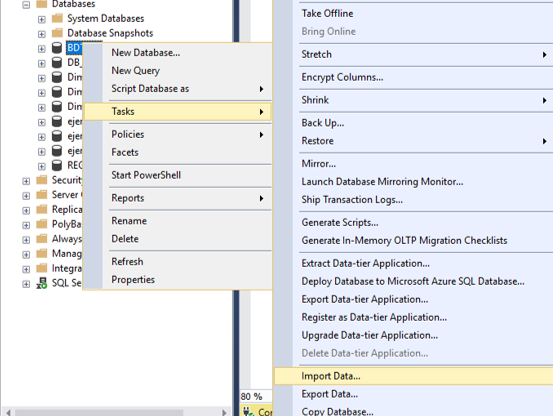
\includegraphics[width=13cm]{./Imagenes/img3}
	\end{center}	

4. Data Source: La base de donde vamos a importar 
	\begin{center}
	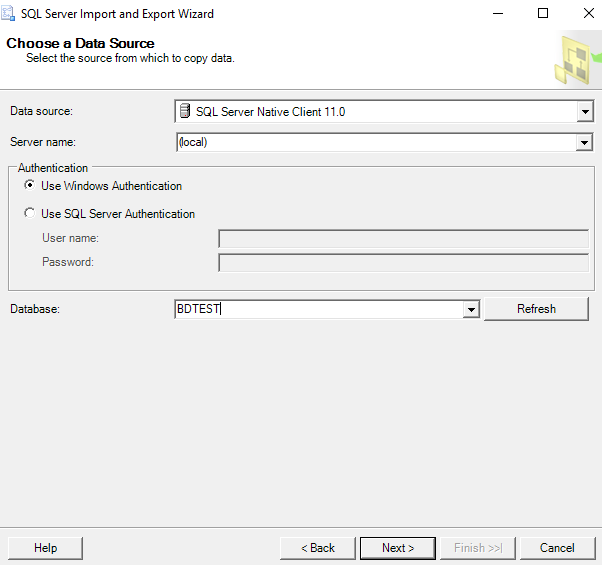
\includegraphics[width=12cm]{./Imagenes/img4}
	\end{center}	
5. Destination: La Base donde vamos a cargar los datos\\
	\begin{center}
	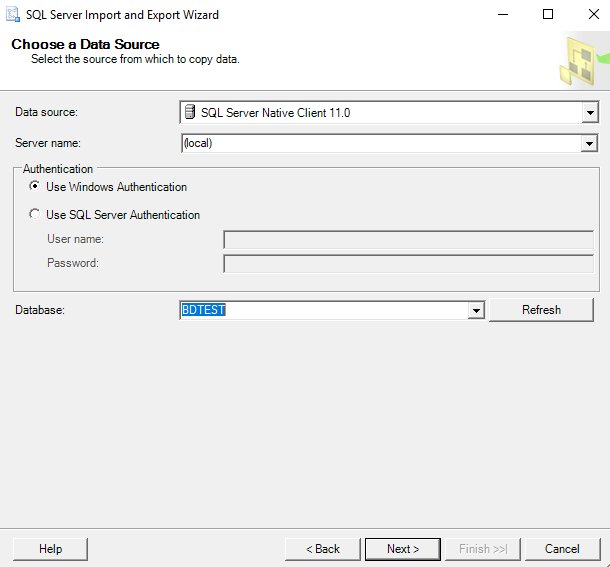
\includegraphics[width=12cm]{./Imagenes/img5}
	\end{center}	
6. Especificar si se realizará copia o consulta, en este caso elejimos copia.\\
	\begin{center}
	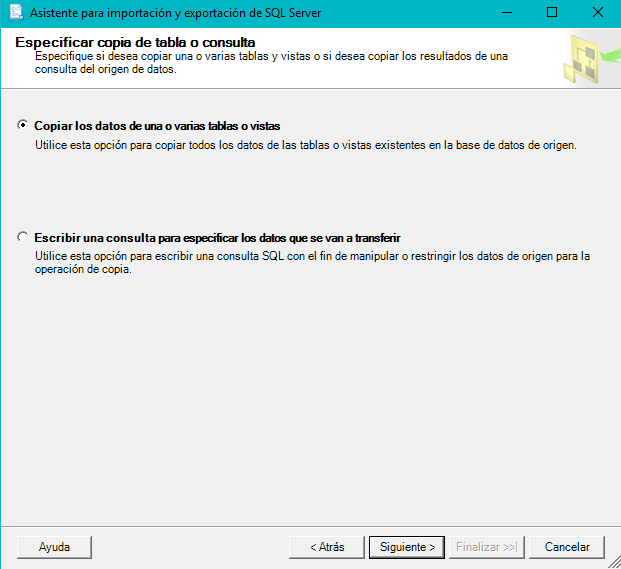
\includegraphics[width=11cm]{./Imagenes/img6}
	\end{center}	
7. Seleccionamos las tablas HumanResources y Person
	\begin{center}
	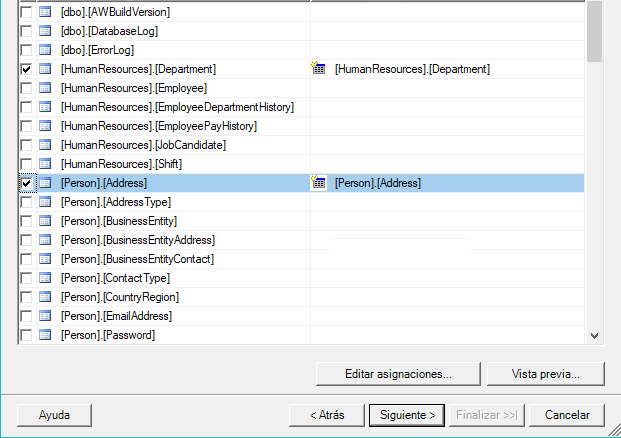
\includegraphics[width=11cm]{./Imagenes/img7}
	\end{center}	
8. Guardamos y ejecutamos.
	\begin{center}
	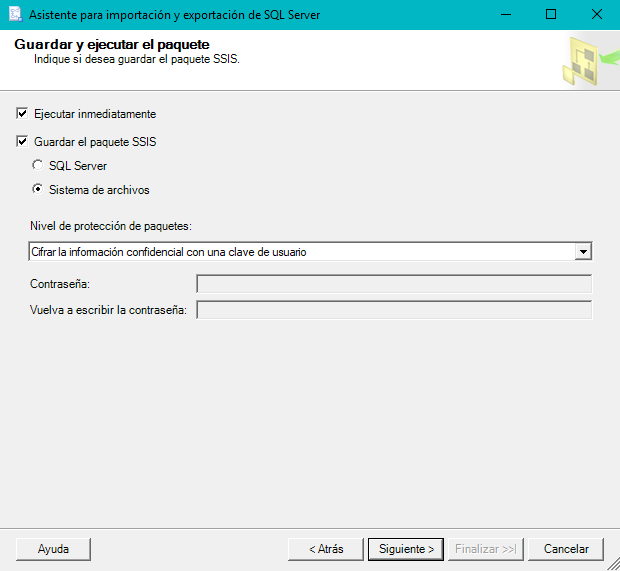
\includegraphics[width=11cm]{./Imagenes/img8}
	\end{center}	
	\begin{center}
	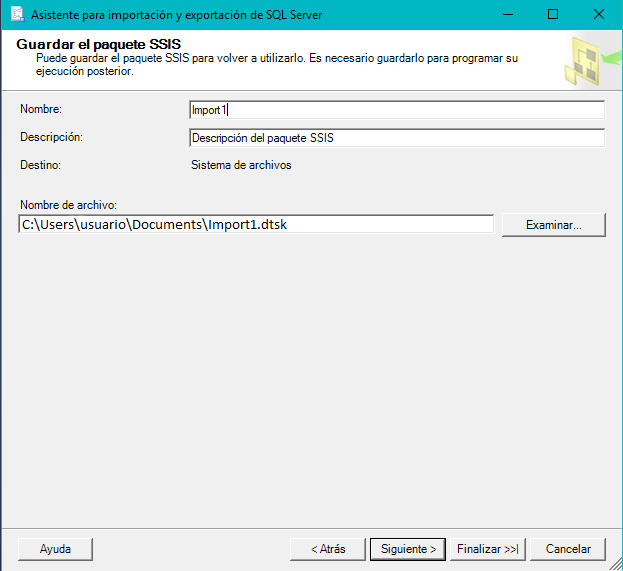
\includegraphics[width=11cm]{./Imagenes/img9}
	\end{center}	
	\begin{center}
	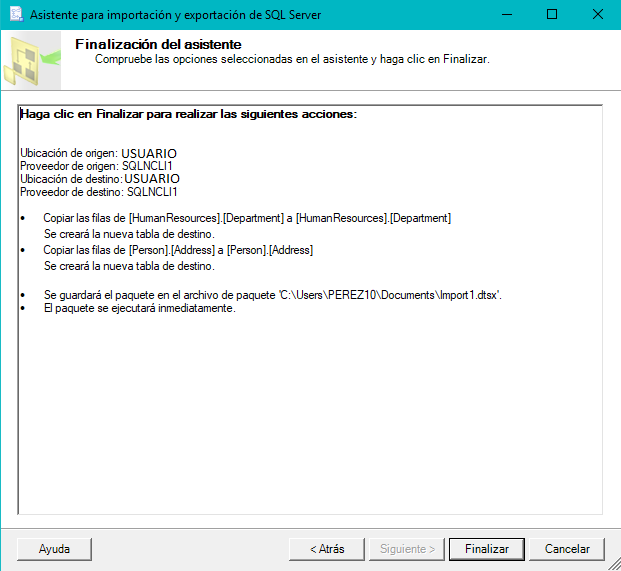
\includegraphics[width=11cm]{./Imagenes/img10}
	\end{center}	

	\begin{center}
	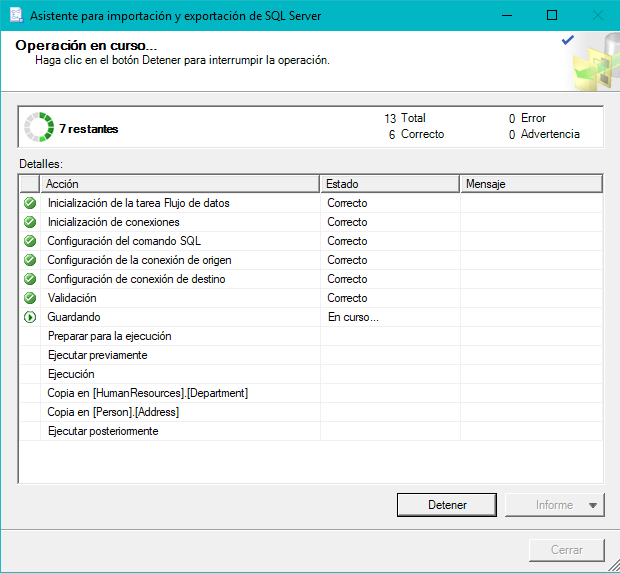
\includegraphics[width=11cm]{./Imagenes/img11}
	\end{center}	
5. Se observa que se realizó correctamente  la ejecución\\
	\begin{center}
	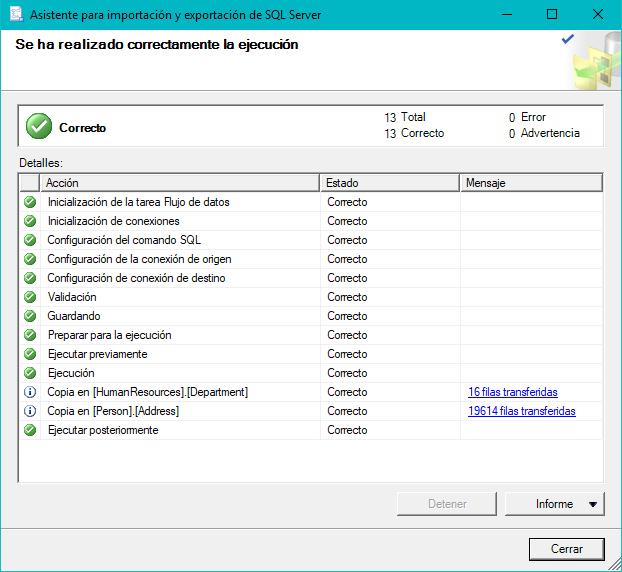
\includegraphics[width=11cm]{./Imagenes/img12}
	\end{center}	 
\section{Actividad 02: Creación del  paquete DTSX} 


1. Abrimos un nuevo Proyecto en nuestro Visual Studio\\
	\begin{center}
	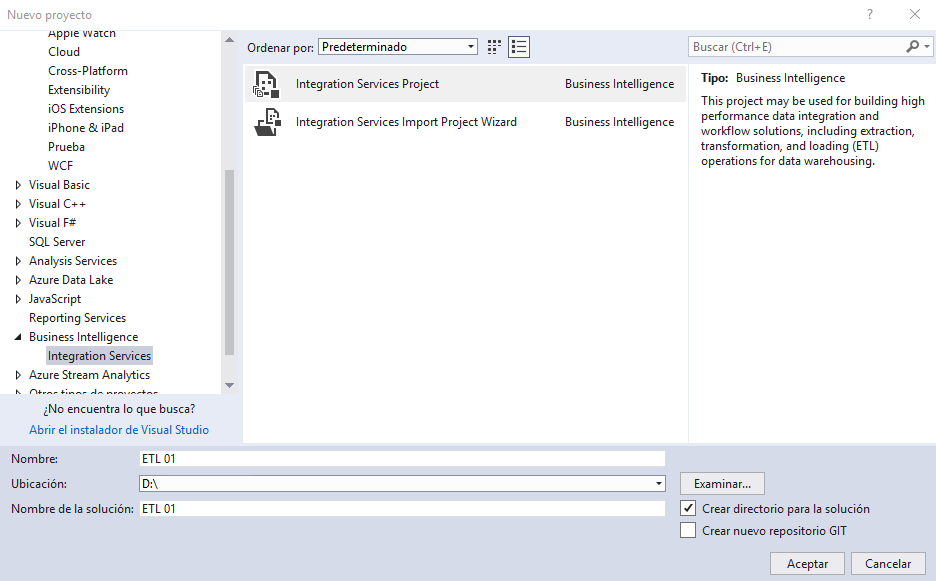
\includegraphics[width=13cm]{./Imagenes/img13}
	\end{center}	

2. En al ventana nueva, sección Solución Explorer, Agrego el paquete generado antes\\
	\begin{center}
	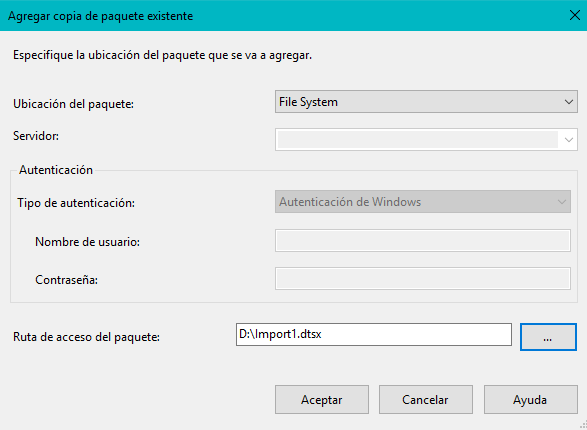
\includegraphics[width=13cm]{./Imagenes/img14}
	\end{center}	
	\begin{center}
	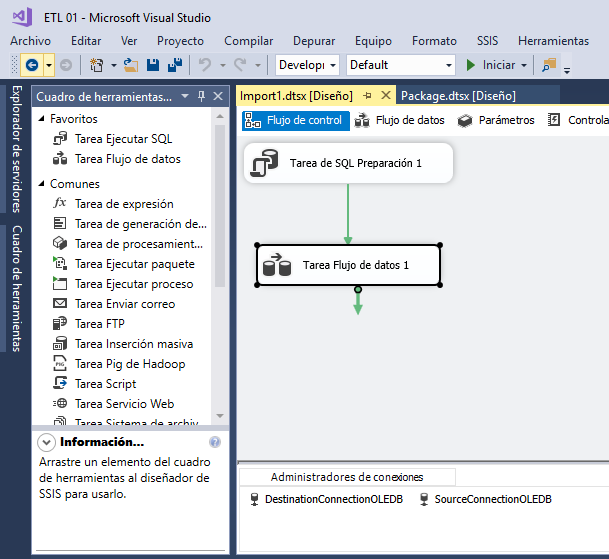
\includegraphics[width=12cm]{./Imagenes/img15}
	\end{center}	
3. Observamos las caracteristicas obtenidas.\\
	\begin{center}
	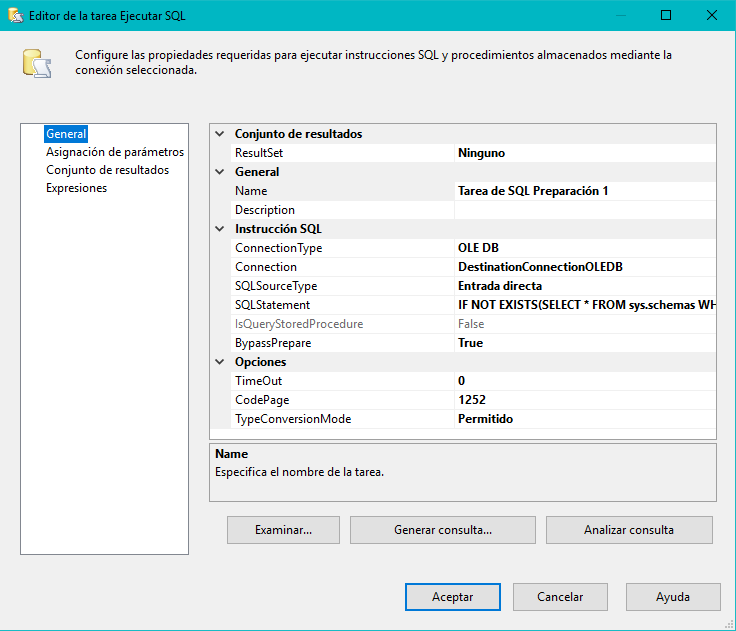
\includegraphics[width=13cm]{./Imagenes/img16}
	\end{center}	

4. En la siguiente ventana mostramos el paquete que se ha importado.\\
	\begin{center}
	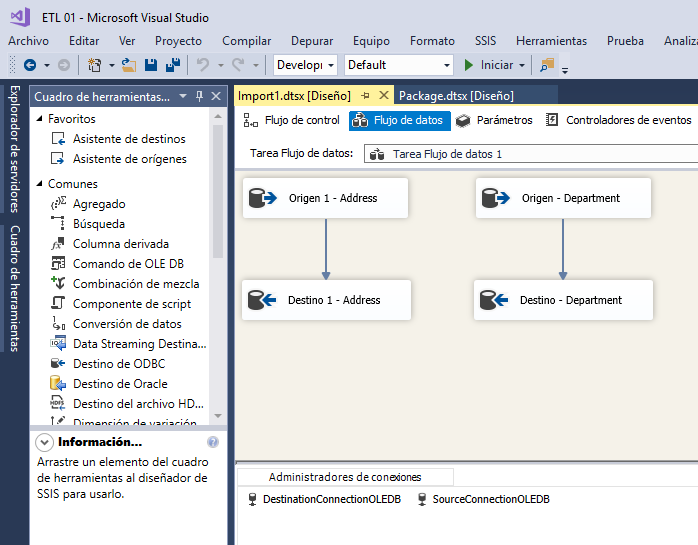
\includegraphics[width=12cm]{./Imagenes/img17}
	\end{center}	
5. Agregamos el administrador de conexiones en este caso el OLEBD. \\
	\begin{center}
	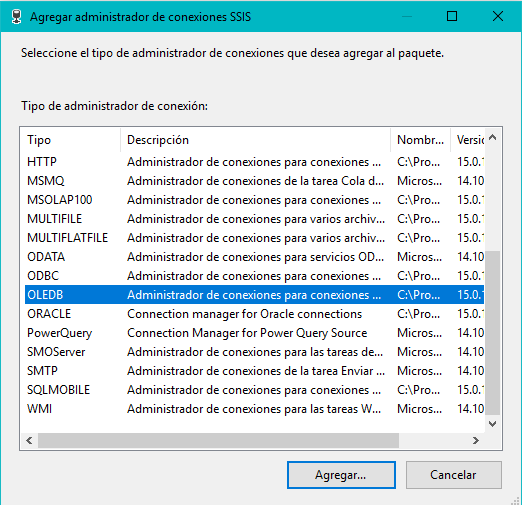
\includegraphics[width=12cm]{./Imagenes/img18}
	\end{center}	

6. En la siguiente ventana mostramos el paquete que se ha importado.\\
	\begin{center}
	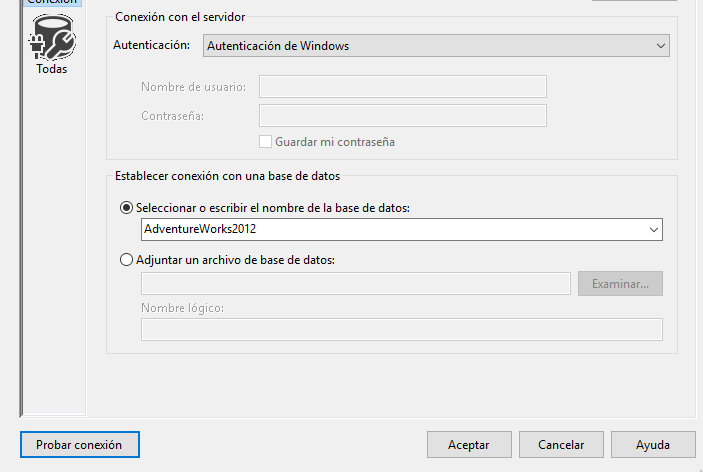
\includegraphics[width=12cm]{./Imagenes/img19}
	\end{center}	
7. Observamos las caracteristicas establecidas.\\
	\begin{center}
	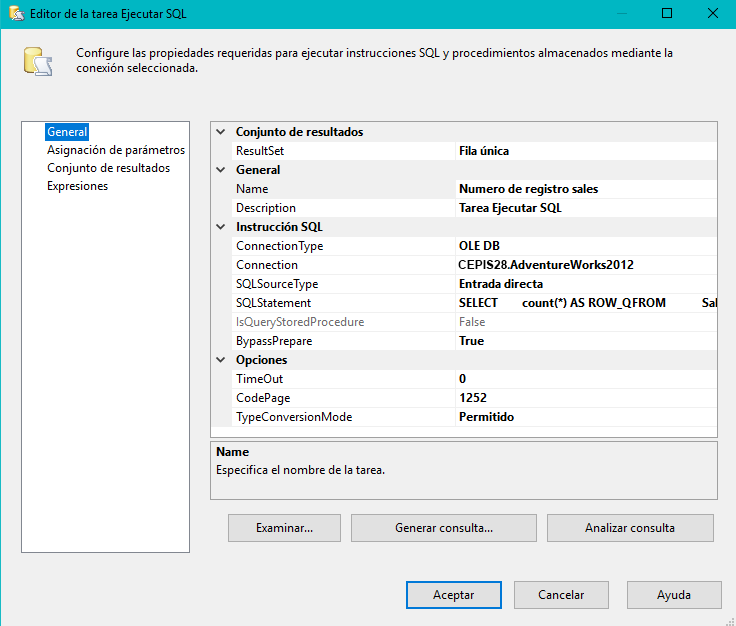
\includegraphics[width=12cm]{./Imagenes/img20}
	\end{center}	
8. Editamos el componente Scrtipt Task Editor.\\
	\begin{center}
	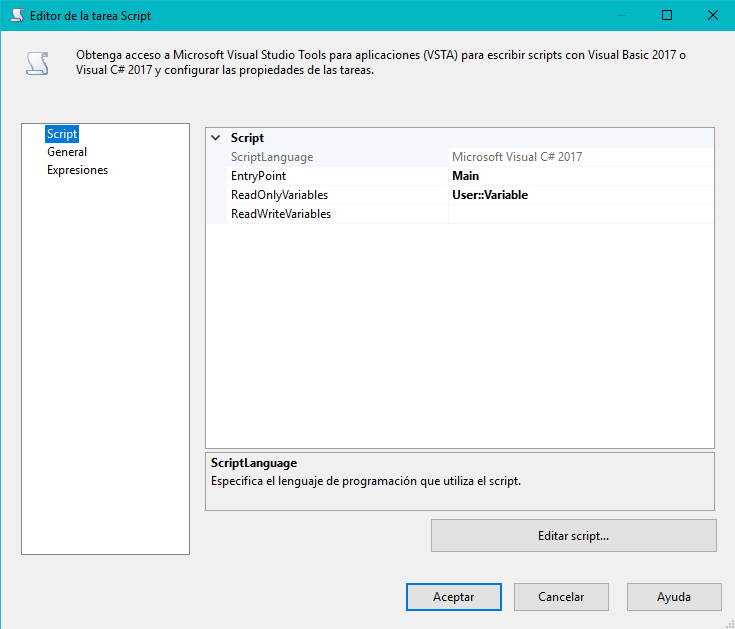
\includegraphics[width=13cm]{./Imagenes/img21}
	\end{center}	
9. El resultado obtenido .\\
	\begin{center}
	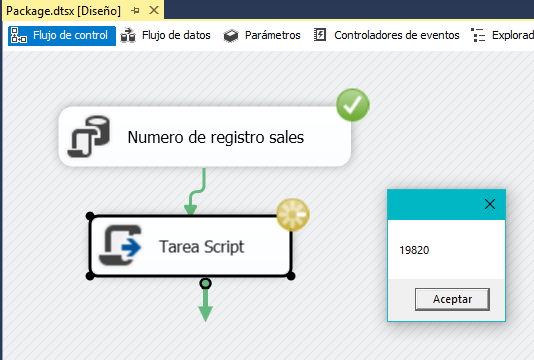
\includegraphics[width=14cm]{./Imagenes/img22}
	\end{center}	
10. Editamos una nueva tarea. \\
	\begin{center}
	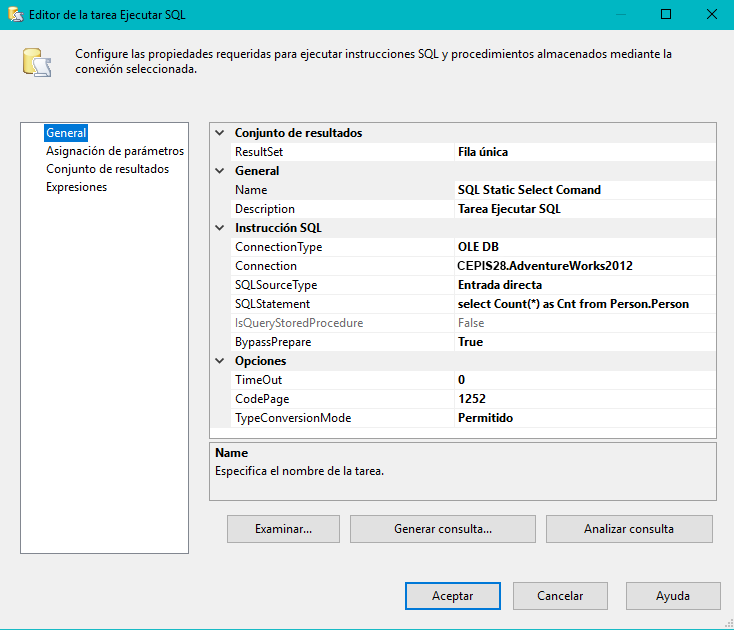
\includegraphics[width=12cm]{./Imagenes/img23}
	\end{center}	
11. Asignacion de parametros. \\
	\begin{center}
	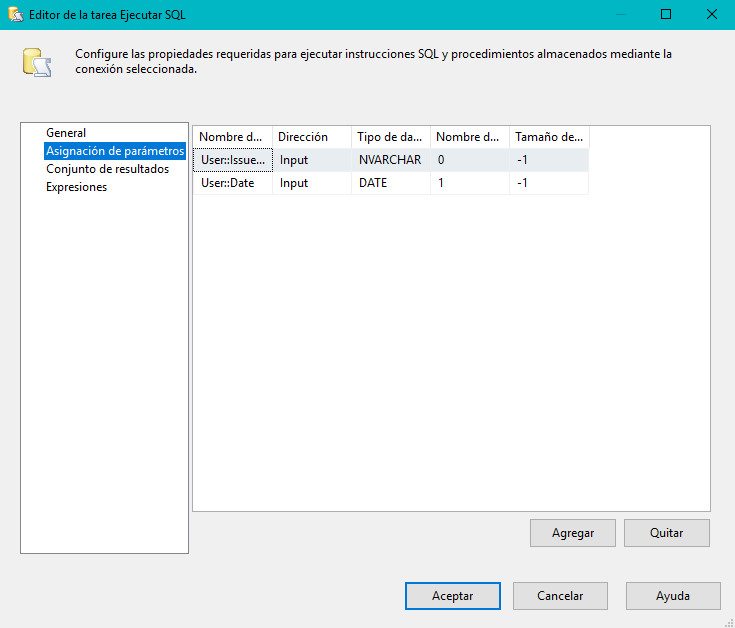
\includegraphics[width=12cm]{./Imagenes/img24}
	\end{center}	

	\begin{center}
	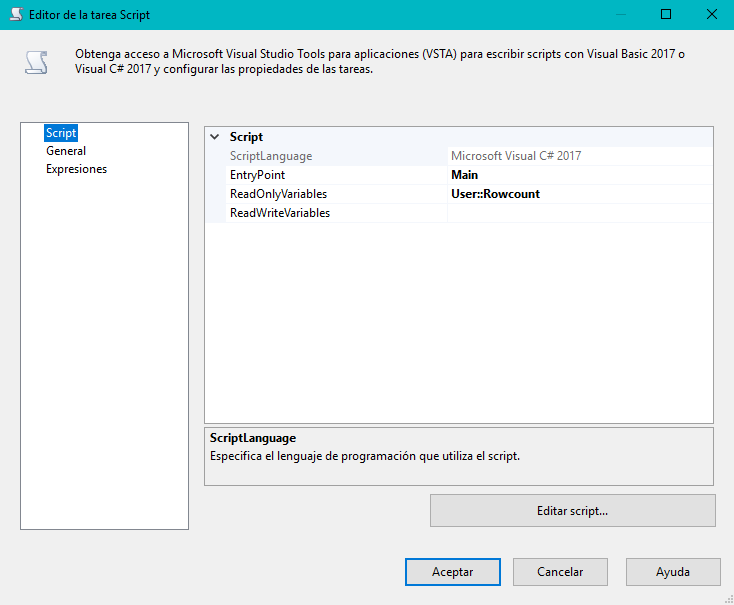
\includegraphics[width=12cm]{./Imagenes/img26}
	\end{center}	
12. Guardamos y los ejecutamos.\\
	\begin{center}
	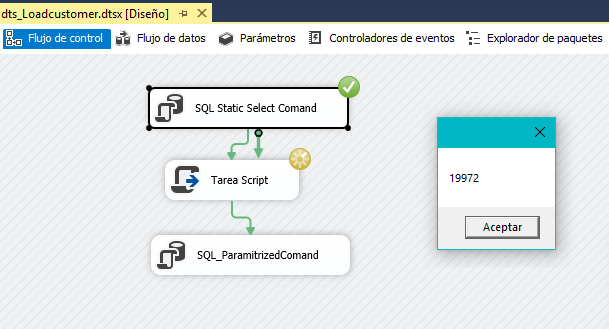
\includegraphics[width=15cm]{./Imagenes/img27}
	\end{center}	 	 	


\end{document}
